\PassOptionsToPackage{unicode=true}{hyperref} % options for packages loaded elsewhere
\PassOptionsToPackage{hyphens}{url}
\PassOptionsToPackage{dvipsnames,svgnames*,x11names*}{xcolor}
%
\documentclass[]{article}
\usepackage{lmodern}
\usepackage{amssymb,amsmath}
\usepackage{ifxetex,ifluatex}
\usepackage{fixltx2e} % provides \textsubscript
\ifnum 0\ifxetex 1\fi\ifluatex 1\fi=0 % if pdftex
  \usepackage[T1]{fontenc}
  \usepackage[utf8]{inputenc}
  \usepackage{textcomp} % provides euro and other symbols
\else % if luatex or xelatex
  \usepackage{unicode-math}
  \defaultfontfeatures{Ligatures=TeX,Scale=MatchLowercase}
\fi
% use upquote if available, for straight quotes in verbatim environments
\IfFileExists{upquote.sty}{\usepackage{upquote}}{}
% use microtype if available
\IfFileExists{microtype.sty}{%
\usepackage[]{microtype}
\UseMicrotypeSet[protrusion]{basicmath} % disable protrusion for tt fonts
}{}
\IfFileExists{parskip.sty}{%
\usepackage{parskip}
}{% else
\setlength{\parindent}{0pt}
\setlength{\parskip}{6pt plus 2pt minus 1pt}
}
\usepackage{xcolor}
\usepackage{hyperref}
\hypersetup{
            pdftitle={Projet de Séries Temporelles},
            pdfauthor={Kim Antunez et Alain Quartier-la-Tente},
            colorlinks=true,
            linkcolor=Maroon,
            filecolor=Maroon,
            citecolor=Blue,
            urlcolor=blue,
            breaklinks=true}
\urlstyle{same}  % don't use monospace font for urls
\usepackage[margin=1in]{geometry}
\usepackage{longtable,booktabs}
% Fix footnotes in tables (requires footnote package)
\IfFileExists{footnote.sty}{\usepackage{footnote}\makesavenoteenv{longtable}}{}
\usepackage{graphicx,grffile}
\makeatletter
\def\maxwidth{\ifdim\Gin@nat@width>\linewidth\linewidth\else\Gin@nat@width\fi}
\def\maxheight{\ifdim\Gin@nat@height>\textheight\textheight\else\Gin@nat@height\fi}
\makeatother
% Scale images if necessary, so that they will not overflow the page
% margins by default, and it is still possible to overwrite the defaults
% using explicit options in \includegraphics[width, height, ...]{}
\setkeys{Gin}{width=\maxwidth,height=\maxheight,keepaspectratio}
\setlength{\emergencystretch}{3em}  % prevent overfull lines
\providecommand{\tightlist}{%
  \setlength{\itemsep}{0pt}\setlength{\parskip}{0pt}}
\setcounter{secnumdepth}{5}
% Redefines (sub)paragraphs to behave more like sections
\ifx\paragraph\undefined\else
\let\oldparagraph\paragraph
\renewcommand{\paragraph}[1]{\oldparagraph{#1}\mbox{}}
\fi
\ifx\subparagraph\undefined\else
\let\oldsubparagraph\subparagraph
\renewcommand{\subparagraph}[1]{\oldsubparagraph{#1}\mbox{}}
\fi

% set default figure placement to htbp
\makeatletter
\def\fps@figure{htbp}
\makeatother

\usepackage{booktabs}
\usepackage{longtable}
\usepackage{array}
\usepackage{multirow}
\usepackage{wrapfig}
\usepackage{float}
\usepackage{colortbl}
\usepackage{pdflscape}
\usepackage{tabu}
\usepackage{threeparttable}
\usepackage{threeparttablex}
\usepackage[normalem]{ulem}
\usepackage{makecell}
\usepackage{xcolor}

\title{Projet de Séries Temporelles}
\author{Kim Antunez et Alain Quartier-la-Tente}
\date{31/03/2020}

\begin{document}
\maketitle

{
\hypersetup{linkcolor=}
\setcounter{tocdepth}{3}
\tableofcontents
}
\hypertarget{partie-1-les-donnuxe9es}{%
\section{Partie 1 : Les données}\label{partie-1-les-donnuxe9es}}

\hypertarget{question-1-description-de-la-suxe9rie-choisie}{%
\subsection{Question 1 : description de la série choisie}\label{question-1-description-de-la-suxe9rie-choisie}}

Pour ce projet, nous avons choisi de travailler sur la série d'indice de production industrielle (IPI) dans l'industrie automobile (identifiant : 010537940).
Il s'agit d'une série au niveau A64 de la nomenclature d'activités française révision 2 (NAF rév. 2), poste CL1.
Cela concerne aussi bien la production des constructeurs de voitures particulières, de véhicules de loisir, de véhicules utilitaires que les équipementiers spécialisés, les carrossiers, les assembleurs ou les prestataires de services d'aménagement de véhicules automobiles.
Cette production intègre donc la filière complète, y compris moteurs et organes mécaniques en amont, dès lors qu'ils sont principalement destinés à des véhicules automobiles (à l'exception des parties de moteur).

C'est un indice de Laspeyres chaîné avec des pondérations annuelles (les pondérations correspondant aux valeurs ajoutées des branches associées).
Il est de base 2015.
L'IPI dans l'industrie automobile est calculé à partir de l'enquête mensuelle de branche, par agrégation de séries ``élémentaires'' calculées à un niveau plus fin.
Ces séries élémentaires sont estimées en volume : la série d'IPI dans l'industrie automobile ne tient donc pas compte des variations de prix.

Les séries de l'IPI sont corrigées des variations saisonnières et des jours ouvrables (CVS-CJO) à partir de la méthode X13-ARIMA.
La désaisonnalisation est réalisée de manière indirecte : elle est effectuée à un niveau fin et les agrégats CVS-CJO sont ensuite calculés directement à partir de ces séries en agrégeant les séries CVS-CJO.
Cette désaisonnalisation est réalisée par sous-périodes pour prendre en compte le fait que la structure économique des séries a beaucoup évolué en 30 ans, et donc qu'il serait peut pertinent d'appliquer un seul modèle de désaisonnalisation sur l'ensemble de la période.
Ainsi, les modèles utilisés pour la désaisonnalisation commencent en 2005 et ces modèles sont utilisées pour estimer les séries CVS-CJO à partir de 2012.

Les séries CVS-CJO avant et après 2012 n'étant pas évalués sur les mêmes modèles, l'idéal serait d'étudier notre série après janvier 2012 pour éviter des ruptures liées à ce changement de modèle. En revanche, cela laisserait une faible profondeur temporelle risquant de fragiliser l'estimation de nos modèles ARIMA.
C'est pourquoi nous allons étudier la série d'IPI dans l'industrie automobile entre \textbf{janvier 2010 et décembre 2019}\footnote{Les derniers points étant souvent sujets à révisions, nous avons préféré ne pas prendre en compte les points de janvier et février 2020.}, c'est-à-dire sur \textbf{120 observations}.

Nous n'effectuerons pas de correction de point atypique ou de transformation logarithmique.

\hypertarget{questions-2-et-3}{%
\subsection{Questions 2 et 3}\label{questions-2-et-3}}

\begin{figure}

{\centering 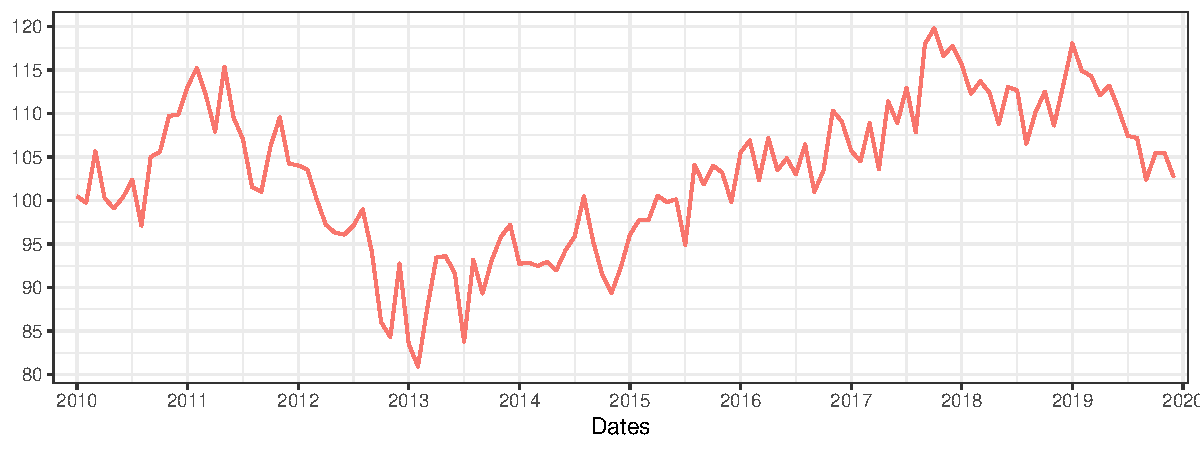
\includegraphics{img/rmd-ipiBrut-1} 

}

\caption{IPI dans l'automobile (CVS-CJO sans traitement)}\label{fig:ipiBrut}
\end{figure}

Le graphique \ref{fig:ipiBrut} ne montre pas de tendance linéaire déterministe nette sur la période 2010-2020 : on observe plutôt une alternance entre des périodes à tendance croissante (2010-2011, 2013-2018) et à tendance décroissante (2011-2013 et 2018-2020).
La série de l'IPI dans l'automobile semble plutôt montrer une tendance stochastique : elle n'est sûrement pas stationnaire. Ceci est vérifié en faisant le test Dickey-Fuller augmenté (ADF) avec une constante non nulle et sans tendance : on ne rejette pas l'hypothèse de présence de racine unitaire au seuil de 5 \% (tableau \ref{tab:tabTestsInit}).
C'est également confirmé par le test de racine unitaire de Phillips-Perron, non rejeté au seuil de 5 \%, et par le test de racine unitaire de Kwiatkowski-Phillips-Schmidt-Shin (KPSS), rejeté au seuil de 5 \% (ici l'hypothèse alternative est la non-stationnarité de la série).

\begin{table}[!h]

\caption{\label{tab:tabTestsInit}Tests de racine unitaire et de stationnarité sur la série d'IPI dans l'automobile}
\centering
\begin{threeparttable}
\begin{tabular}[t]{lccc}
\toprule
Test & Statistique & p-valeur & \\
\midrule
Dickey-Fuller augmenté \textsuperscript{a} & -1.678 & 0.434 & \\
Phillips-Perron & -2.578 & 0.336 & \\
KPSS & 0.892 & 0.010 & **\\
\bottomrule
\end{tabular}
\begin{tablenotes}
\item \hspace{-0.4cm}\textbf{Signif. codes: }0 `***' 0.001 `**' 0.01 `*' 0.05 `.' 0.1 ` ' 1
\item[a] Le test ADF a été fait en rajoutant 2 retards. De cette façon les résidus utilisés dans ce test sont bien indépendants et le test ADF est bien interprétable
\end{tablenotes}
\end{threeparttable}
\end{table}

D'après le graphique \ref{fig:ipiBrut}, la série différenciée semble stationnaire.
C'est confirmé par le test de Dickey-Fuller augmenté, effectué avec une constante nulle et sans tendance, le test de Phillips-Perron et le test KPSS (tableau \ref{tab:tabTestsDiff}).

\begin{table}[!h]

\caption{\label{tab:tabTestsDiff}Tests de racine unitaire et de stationnarité sur la série différenciée d'IPI dans l'automobile}
\centering
\begin{threeparttable}
\begin{tabular}[t]{lccc}
\toprule
Test & Statistique & p-valeur & \\
\midrule
Dickey-Fuller augmenté \textsuperscript{a} & -10.261 & 0.010 & **\\
Phillips-Perron & -15.132 & 0.010 & **\\
KPSS & 0.074 & 0.100 & .\\
\bottomrule
\end{tabular}
\begin{tablenotes}
\item \hspace{-0.4cm}\textbf{Signif. codes: }0 `***' 0.001 `**' 0.01 `*' 0.05 `.' 0.1 ` ' 1
\item[a] Le test ADF a été fait en rajoutant 1 retard. De cette façon les résidus utilisés dans ce test sont bien indépendants et le test ADF est bien interprétable
\end{tablenotes}
\end{threeparttable}
\end{table}

\begin{figure}

{\centering 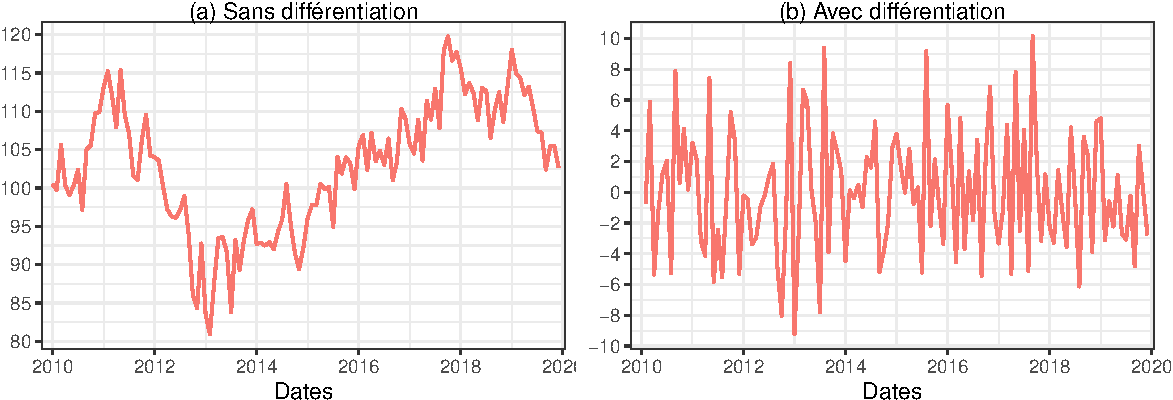
\includegraphics{img/rmd-compGraph-1} 

}

\caption{IPI dans l'automobile (CVS-CJO) sans et avec différentiation}\label{fig:compGraph}
\end{figure}

\hypertarget{partie-2-moduxe8les-arima}{%
\section{Partie 2 : Modèles ARIMA}\label{partie-2-moduxe8les-arima}}

Pour déterminer les ordres maximaux, \(p_{max}\) et \(q_{max}\), du modèle \(ARMA(p,q)\) suivi par la série différenciée de l'IPI dans l'automobile, analysons les autocorrélogrammes et les autocorrélogrammes partiels (graphique \ref{fig:acfPacf}).
À partir de retard 2 (inclus), tous les autocorrélogrammes ne sont pas significatifs à 5 \% : on en déduit que \(p_{max} = 1\).
À partir de retard 2 (inclus), tous les autocorrélogrammes partiels ne sont pas significatifs à 5 \% : on en déduit que \(q_{max} = 1\).\\
Ainsi, pour savoir quel modèle choisir nous allons tester tous les modèles \(ARMA(p,q)\) tels que \(p\leq 1\) et \(q\leq 1\).

\begin{figure}

{\centering 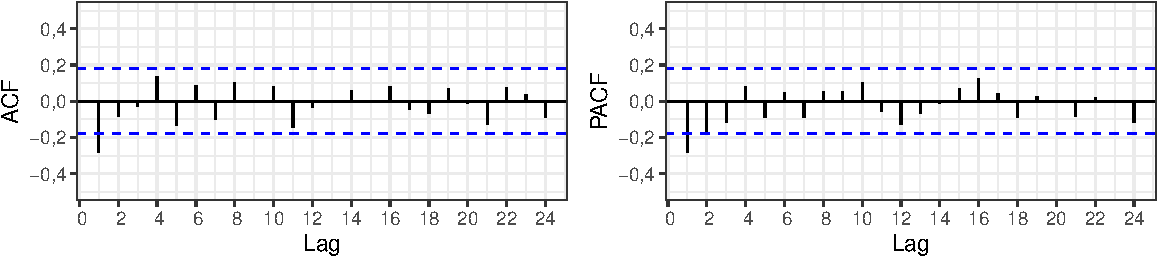
\includegraphics{img/rmd-acfPacf-1} 

}

\caption{Autocorrélogrammes (ACF) et autocorrélogrammes partiels (PACF) pour la série différenciée de l'IPI dans l'automobile}\label{fig:acfPacf}
\end{figure}

Quatre modèles ARMA ont été testés, ils ont été estimés sans constante :

\begin{itemize}
\item
  \emph{ARMA(0,0)} : les résidus de ce modèle ne sont pas indépendants (tableau \ref{tab:tablbtest}) -\textgreater{} \textbf{modèle non retenu}
\item
  \emph{ARMA(1,0)} : les résidus de ce modèle ne sont pas indépendants (tableau \ref{tab:tablbtest}) -\textgreater{} \textbf{modèle non retenu}
\item
  \emph{ARMA(0,1)} : les résidus de ce modèle sont indépendants (tableau \ref{tab:tablbtest}) et le coefficient associé au MA(1) est significatif (tableau \ref{tab:tabcoefs}) -\textgreater{} \textbf{modèle retenu}
\item
  \emph{ARMA(1,1)} : les résidus de ce modèle sont indépendants (tableau \ref{tab:tablbtest}) mais le coefficient associé au AR(1) n'est significatif (tableau \ref{tab:tabcoefs}) -\textgreater{} \textbf{modèle non retenu}
\end{itemize}

En somme, il n'y a qu'un seul modèle ARMA valide sur l'IPI différencié : c'est le modèle ARMA(0,1).
Pour l'IPI automobile, \(X_t\) on retient donc le modèle ARIMA(0,1,1) suivant :
\[
\Delta X_t = \varepsilon_t - \underset{(0,09)}{0,38}\;\varepsilon_{t-1}
\]
\(\varepsilon_t\) est bien un bruit blanc : les \((\varepsilon_t)_t\) sont indépendants (tableau \ref{tab:tablbtest}), homoscédastiques (tableau \ref{tab:tablb2test}) et suivent aussi une loi normale (tableau \ref{tab:tabjb}).

Parmi l'ensemble des modèles testés, l'ARIMA(0,1,1) est aussi le modèle qui minimise les critères d'information (tableau \ref{tab:aicbic}).

\begin{table}[!h]

\caption{\label{tab:aicbic}Critères d'information des modèles ARIMA sur l'IPI de l'automobile}
\centering
\begin{tabular}[t]{lcccc}
\toprule
  & ARIMA(0,1,0) & ARIMA(1,1,0) & ARIMA(0,1,1) & ARIMA(1,1,1)\\
\midrule
AIC & 672.439 & 664.677 & 660.932 & 662.345\\
BIC & 675.219 & 670.235 & 666.490 & 670.683\\
\bottomrule
\end{tabular}
\end{table}

\hypertarget{partie-3-pruxe9visions}{%
\section{Partie 3 : Prévisions}\label{partie-3-pruxe9visions}}

\hypertarget{question-6-7-et-8-construction-dun-intervalle-de-confiance}{%
\subsection{Question 6, 7 et 8 : construction d'un intervalle de confiance}\label{question-6-7-et-8-construction-dun-intervalle-de-confiance}}

On cherche désormais à faire une prévision de \(X_t\) à l'horizon \(T+2\).
Notons \(\hat\theta_1\) le coefficient associé à la partie MA de notre modèle ARMA(0,1,1), estimé entre janvier 2010 et décembre 2019 (\(\hat\theta_1\simeq -0,38\)). On a :
\[
\Delta X_T = \varepsilon_T + \hat\theta_1\varepsilon_{T-1}
\iff 
X_T = X_{T-1} + \varepsilon_T + \hat\theta_1\varepsilon_{T-1}
\]
Les prévisions de \(X_{T+1}\) et \(X_{T+2}\) réalisées à l'instant \(T\), notées \(\hat X_{T+1\vert T}\) et \(\hat X_{T+2\vert T}\), vérifient donc l'équation :
\[
\begin{cases}
\hat X_{T+1\vert T}=X_T - \hat\theta_1\varepsilon_T \\
\hat X_{T+2\vert T}=\hat X_{T+1\vert T}
\end{cases}
\]
Les erreurs de prévision sont égales à :
\[
\begin{cases}
\hat \varepsilon_{T+1\vert T} = X_{T+1} - \hat X_{T+1\vert T}=
\varepsilon_{T+1}+(\theta_1-\hat\theta_1)\varepsilon_T
\\
\hat \varepsilon_{T+2\vert T} = X_{T+2} - \hat X_{T+2\vert T}=
\varepsilon_{T+2}+(1+\theta_1)\varepsilon_{T+1}+(\theta_1-\hat\theta_1)\varepsilon_T 
\end{cases}
\]
Les intervalles de confiance de niveau \(\alpha\) sur \(\hat X_{T+1\vert T}\) et \(\hat X_{T+2\vert T}\) s'écrivent donc :
\[
IC_{1-\alpha}(\hat X_{T+h\vert T}) =
\left[
\hat X_{T+h\vert T}-q_{1-\frac \alpha 2}\hat{\sigma}_h\;;\;
\hat X_{T+h\vert T}+q_{1-\frac \alpha 2}\hat{\sigma}_h
\right]
\]
Avec \(q_{1-\frac \alpha 2}\) le quantile \(1-\frac \alpha 2\) d'une loi \(\mathcal N(0,1)\) et :
\[
\hat \sigma_1 = \hat\sigma\text{,}\quad
\hat\sigma_2=\hat\sigma\sqrt{1+(1+\hat \theta_1)^2}\quad\text{et}
\quad 
\hat\sigma = \frac{1}{T-2}\sum_{t=2}^T\hat\varepsilon_t^2
\]
(la somme commence à 2 puisque l'on perd une période en différenciant)

Bilan :
\begin{equation}
IC_{1-\alpha}\left(\begin{pmatrix} \hat X_{T+1\vert T}
\\ \hat X_{T+2\vert T}\end{pmatrix}\right) =
\left[
  \begin{pmatrix} 
    X_T - \hat\theta_1\varepsilon_T 
    \\ X_T - \hat\theta_1\varepsilon_T 
  \end{pmatrix}
  -
  \hat\sigma q_{1-\frac \alpha 2}
  \begin{pmatrix} 
    1\\
    \sqrt{1+(1+\hat \theta_1)^2}
  \end{pmatrix}
  \;;\;
  \begin{pmatrix} 
    X_T - \hat\theta_1\varepsilon_T 
    \\ X_T - \hat\theta_1\varepsilon_T 
  \end{pmatrix}
  +
  \hat\sigma q_{1-\frac \alpha 2}
  \begin{pmatrix} 
    1\\
    \sqrt{1+(1+\hat \theta_1)^2}
  \end{pmatrix}
\right]
\label{eq:icPrev}
\end{equation}

Pour obtenir ces intervalles de confiance il faut que les résidus de notre modèle ARIMA soient indépendants, homoscédastiques et suivent une loi normale : ce qui est bien vérifié dans notre cas.

Le graphique XXX montre cette région de confiance au seuil 95 \%, ainsi que les valeurs actuelles de l'IPI automobile de janvier et de février 2020.
On retrouve ce que l'on a montré par l'équation \eqref{eq:icPrev} : on prévoit la même valeur en \(X_{T+1}\) et \(X_{T+2}\) et plus l'horizon augmente plus l'incertitude autour de la prévision (i.e : l'intervalle de confiance) augmente.
Cela parait peu cohérent économiquement de garder la même prévision pour les deux dates mais cela reflète la dynamique du modèle ARIMA(0,1,1) :

\begin{itemize}
\item
  Puisqu'il y a aucun ordre autorégressif, \(\Delta X_t\) ne dépend pas des valeurs passées prises par \((\Delta X_{t'})_{t'\leq t-1}\).
\item
  Puisque l'ordre MA est égale à 1, il n'y a aucune influence du bruit à l'horizon supérieur ou égal à 2 : sans aucune information supplémentaire, la seule prévision possible pour \(\Delta X_{t+h}\), \(h\geq 2\), est une prévision nulle, et donc pour \(X_{t+h}\) la seule prévision possible est \(\hat X_{t+1\vert t}\).
  Cette incertitude se traduit par une rapide augmentation de l'intervalle de confiance.
\end{itemize}

\hypertarget{question-9-question-ouverte}{%
\subsection{Question 9 : question ouverte}\label{question-9-question-ouverte}}

Granger

\hypertarget{appendix-appendix}{%
\appendix}


\hypertarget{sec:qualRes}{%
\section{Annexe 1 : tests supplémentaires sur la qualité des modèles}\label{sec:qualRes}}

\begin{table}[!h]

\caption{\label{tab:tablbtest}Tests de Ljung-Box sur les résidus (tests d'autocorrélation) des modèles ARIMA sur l'IPI de l'automobile}
\centering
\resizebox{\linewidth}{!}{
\begin{threeparttable}
\begin{tabular}[t]{ccccccccccccc}
\toprule
\multicolumn{1}{c}{ } & \multicolumn{2}{c}{ARIMA(0,1,0)} & \multicolumn{1}{c}{ } & \multicolumn{2}{c}{ARIMA(1,1,0)} & \multicolumn{1}{c}{ } & \multicolumn{2}{c}{ARIMA(0,1,1)} & \multicolumn{1}{c}{ } & \multicolumn{2}{c}{ARIMA(1,1,1)} & \multicolumn{1}{c}{ } \\
\cmidrule(l{3pt}r{3pt}){2-3} \cmidrule(l{3pt}r{3pt}){5-6} \cmidrule(l{3pt}r{3pt}){8-9} \cmidrule(l{3pt}r{3pt}){11-12}
Retards & Statistique & p-valeur &  & Statistique & p-valeur &  & Statistique & p-valeur &  & Statistique & p-valeur & \\
\midrule
1 & 9.652 & 0.002 & ** &  &  &  &  &  &  &  &  & \\
2 & 10.473 & 0.005 & ** & 4.757 & 0.029 & * & 0.858 & 0.354 &  &  &  & \\
3 & 10.580 & 0.014 & * & 4.796 & 0.091 & . & 0.925 & 0.630 &  & 0.106 & 0.744 & \\
4 & 12.843 & 0.012 & * & 6.191 & 0.103 &  & 1.985 & 0.576 &  & 1.544 & 0.462 & \\
5 & 15.122 & 0.010 & ** & 7.239 & 0.124 &  & 3.024 & 0.554 &  & 2.606 & 0.456 & \\
\addlinespace
6 & 16.041 & 0.014 & * & 7.327 & 0.197 &  & 3.165 & 0.675 &  & 2.907 & 0.573 & \\
7 & 17.341 & 0.015 & * & 7.800 & 0.253 &  & 3.566 & 0.735 &  & 3.389 & 0.640 & \\
8 & 18.808 & 0.016 & * & 8.936 & 0.257 &  & 4.884 & 0.674 &  & 4.676 & 0.586 & \\
9 & 18.809 & 0.027 & * & 9.306 & 0.317 &  & 5.129 & 0.744 &  & 4.781 & 0.687 & \\
10 & 19.645 & 0.033 & * & 9.610 & 0.383 &  & 5.338 & 0.804 &  & 5.037 & 0.754 & \\
\addlinespace
11 & 22.433 & 0.021 & * & 12.895 & 0.230 &  & 8.684 & 0.562 &  & 8.103 & 0.524 & \\
12 & 22.609 & 0.031 & * & 13.822 & 0.243 &  & 9.649 & 0.562 &  & 8.787 & 0.552 & \\
13 & 22.610 & 0.047 & * & 13.838 & 0.311 &  & 9.649 & 0.647 &  & 8.787 & 0.642 & \\
14 & 23.078 & 0.059 & . & 14.496 & 0.340 &  & 10.455 & 0.656 &  & 9.497 & 0.660 & \\
15 & 23.082 & 0.082 & . & 14.860 & 0.388 &  & 11.003 & 0.686 &  & 9.871 & 0.704 & \\
\addlinespace
16 & 24.077 & 0.088 & . & 15.947 & 0.386 &  & 12.232 & 0.661 &  & 11.074 & 0.680 & \\
17 & 24.339 & 0.111 &  & 16.263 & 0.435 &  & 12.411 & 0.715 &  & 11.227 & 0.736 & \\
18 & 24.935 & 0.127 &  & 16.911 & 0.460 &  & 12.993 & 0.737 &  & 11.795 & 0.758 & \\
19 & 25.633 & 0.141 &  & 17.430 & 0.494 &  & 13.173 & 0.781 &  & 11.966 & 0.802 & \\
20 & 25.649 & 0.178 &  & 17.579 & 0.551 &  & 13.432 & 0.816 &  & 12.208 & 0.836 & \\
\addlinespace
21 & 28.080 & 0.138 &  & 20.078 & 0.453 &  & 15.782 & 0.730 &  & 14.643 & 0.745 & \\
22 & 28.992 & 0.145 &  & 20.694 & 0.478 &  & 16.064 & 0.766 &  & 14.878 & 0.783 & \\
23 & 29.209 & 0.173 &  & 20.920 & 0.526 &  & 16.146 & 0.809 &  & 14.914 & 0.827 & \\
24 & 30.464 & 0.170 &  & 21.907 & 0.526 &  & 17.136 & 0.803 &  & 16.104 & 0.811 & \\
\bottomrule
\end{tabular}
\begin{tablenotes}
\item \hspace{-0.4cm}\textbf{Signif. codes: }0 `***' 0.001 `**' 0.01 `*' 0.05 `.' 0.1 ` ' 1
\end{tablenotes}
\end{threeparttable}}
\end{table}

\begin{table}[!h]

\caption{\label{tab:tablb2test}Tests de Ljung-Box sur le carré des résidus (tests d'homoscédasticité) des modèles ARIMA sur l'IPI de l'automobile}
\centering
\resizebox{\linewidth}{!}{
\begin{threeparttable}
\begin{tabular}[t]{ccccccccccccc}
\toprule
\multicolumn{1}{c}{ } & \multicolumn{2}{c}{ARIMA(0,1,0)} & \multicolumn{1}{c}{ } & \multicolumn{2}{c}{ARIMA(1,1,0)} & \multicolumn{1}{c}{ } & \multicolumn{2}{c}{ARIMA(0,1,1)} & \multicolumn{1}{c}{ } & \multicolumn{2}{c}{ARIMA(1,1,1)} & \multicolumn{1}{c}{ } \\
\cmidrule(l{3pt}r{3pt}){2-3} \cmidrule(l{3pt}r{3pt}){5-6} \cmidrule(l{3pt}r{3pt}){8-9} \cmidrule(l{3pt}r{3pt}){11-12}
Retards & Statistique & p-valeur &  & Statistique & p-valeur &  & Statistique & p-valeur &  & Statistique & p-valeur & \\
\midrule
1 & 2.832 & 0.092 & . &  &  &  &  &  &  &  &  & \\
2 & 2.843 & 0.241 &  & 2.917 & 0.088 & . & 2.032 & 0.154 &  &  &  & \\
3 & 2.860 & 0.414 &  & 3.844 & 0.146 &  & 3.569 & 0.168 &  & 3.140 & 0.076 & .\\
4 & 3.227 & 0.521 &  & 5.425 & 0.143 &  & 4.164 & 0.244 &  & 3.575 & 0.167 & \\
5 & 3.233 & 0.664 &  & 5.448 & 0.244 &  & 4.183 & 0.382 &  & 3.576 & 0.311 & \\
\addlinespace
6 & 3.262 & 0.775 &  & 7.479 & 0.187 &  & 6.916 & 0.227 &  & 5.513 & 0.239 & \\
7 & 3.263 & 0.860 &  & 7.836 & 0.250 &  & 7.515 & 0.276 &  & 6.127 & 0.294 & \\
8 & 3.270 & 0.916 &  & 8.294 & 0.307 &  & 7.781 & 0.352 &  & 6.290 & 0.392 & \\
9 & 3.772 & 0.926 &  & 8.613 & 0.376 &  & 7.787 & 0.455 &  & 6.314 & 0.504 & \\
10 & 3.797 & 0.956 &  & 8.727 & 0.463 &  & 7.838 & 0.551 &  & 6.605 & 0.580 & \\
\addlinespace
11 & 5.286 & 0.917 &  & 9.343 & 0.500 &  & 8.071 & 0.622 &  & 6.897 & 0.648 & \\
12 & 5.482 & 0.940 &  & 10.431 & 0.492 &  & 9.136 & 0.609 &  & 7.987 & 0.630 & \\
13 & 5.619 & 0.959 &  & 11.058 & 0.524 &  & 9.537 & 0.656 &  & 8.373 & 0.680 & \\
14 & 7.532 & 0.912 &  & 12.221 & 0.510 &  & 10.714 & 0.635 &  & 9.807 & 0.633 & \\
15 & 7.727 & 0.934 &  & 12.252 & 0.586 &  & 10.784 & 0.703 &  & 9.807 & 0.710 & \\
\addlinespace
16 & 7.760 & 0.956 &  & 12.256 & 0.660 &  & 10.802 & 0.766 &  & 9.823 & 0.775 & \\
17 & 7.866 & 0.969 &  & 12.268 & 0.725 &  & 10.968 & 0.811 &  & 9.890 & 0.827 & \\
18 & 11.403 & 0.876 &  & 12.791 & 0.750 &  & 11.573 & 0.825 &  & 11.468 & 0.780 & \\
19 & 11.440 & 0.908 &  & 12.791 & 0.804 &  & 11.788 & 0.858 &  & 11.709 & 0.817 & \\
20 & 12.066 & 0.914 &  & 13.115 & 0.833 &  & 12.156 & 0.879 &  & 12.086 & 0.843 & \\
\addlinespace
21 & 12.213 & 0.934 &  & 14.050 & 0.828 &  & 13.228 & 0.867 &  & 12.984 & 0.839 & \\
22 & 13.751 & 0.910 &  & 15.070 & 0.819 &  & 14.231 & 0.859 &  & 14.364 & 0.812 & \\
23 & 14.907 & 0.898 &  & 15.242 & 0.852 &  & 14.284 & 0.891 &  & 14.389 & 0.852 & \\
24 & 15.944 & 0.890 &  & 16.450 & 0.835 &  & 16.650 & 0.826 &  & 16.688 & 0.780 & \\
\bottomrule
\end{tabular}
\begin{tablenotes}
\item \hspace{-0.4cm}\textbf{Signif. codes: }0 `***' 0.001 `**' 0.01 `*' 0.05 `.' 0.1 ` ' 1
\end{tablenotes}
\end{threeparttable}}
\end{table}

\begin{table}[!h]

\caption{\label{tab:tabjb}Tests de Jarque-Bera de normalité des résidus des modèles ARIMA sur l'IPI de l'automobile}
\centering
\begin{threeparttable}
\begin{tabular}[t]{lccc}
\toprule
  & Statistique & p-valeur & \\
\midrule
ARIMA(0,1,0) & 2.381 & 0.304 & \\
ARIMA(1,1,0) & 2.414 & 0.299 & \\
ARIMA(0,1,1) & 2.363 & 0.307 & \\
ARIMA(1,1,1) & 2.241 & 0.326 & \\
\bottomrule
\end{tabular}
\begin{tablenotes}
\item \hspace{-0.4cm}\textbf{Signif. codes: }0 `***' 0.001 `**' 0.01 `*' 0.05 `.' 0.1 ` ' 1
\item Le test de Jarque-Bera suppose que les résidus soient indépendants et homoscédastiques
\end{tablenotes}
\end{threeparttable}
\end{table}

\begin{table}[!h]

\caption{\label{tab:tabcoefs}Estimation des coefficients associés aux modèles ARIMA sur l'IPI de l'automobile}
\centering
\begin{threeparttable}
\begin{tabular}[t]{lcccccccc}
\toprule
\multicolumn{1}{c}{ } & \multicolumn{3}{c}{AR(1)} & \multicolumn{1}{c}{ } & \multicolumn{3}{c}{MA(1)} & \multicolumn{1}{c}{ } \\
\cmidrule(l{3pt}r{3pt}){2-4} \cmidrule(l{3pt}r{3pt}){6-8}
  & Coefficient & Écart-type & p-valeur &  & Coefficient & Écart-type & p-valeur & \\
\midrule
ARIMA(0,1,0) &  &  &  &  &  &  &  & \\
ARIMA(1,1,0) & -0.280 & 0.088 & 0.001 & ** &  &  &  & \\
ARIMA(0,1,1) &  &  &  &  & -0.377 & 0.091 & 0.000 & ***\\
ARIMA(1,1,1) & 0.165 & 0.214 & 0.439 &  & -0.515 & 0.183 & 0.005 & **\\
\bottomrule
\end{tabular}
\begin{tablenotes}
\item \hspace{-0.4cm}\textbf{Signif. codes: }0 `***' 0.001 `**' 0.01 `*' 0.05 `.' 0.1 ` ' 1
\end{tablenotes}
\end{threeparttable}
\end{table}

\end{document}
